% Created 2021-05-26 Wed 16:21
% Intended LaTeX compiler: pdflatex
\documentclass[11pt]{article}
\usepackage[utf8]{inputenc}
\usepackage[T1]{fontenc}
\usepackage{graphicx}
\usepackage{grffile}
\usepackage{longtable}
\usepackage{wrapfig}
\usepackage{rotating}
\usepackage[normalem]{ulem}
\usepackage{amsmath}
\usepackage{textcomp}
\usepackage{amssymb}
\usepackage{capt-of}
\usepackage{hyperref}
\author{Garrett Finucane}
\date{\today}
\title{Density and Neutral Variables}
\hypersetup{
 pdfauthor={Garrett Finucane},
 pdftitle={Density and Neutral Variables},
 pdfkeywords={},
 pdfsubject={},
 pdfcreator={Emacs 27.2 (Org mode 9.4.4)}, 
 pdflang={English}}
\begin{document}

\maketitle
\tableofcontents



\section{Who is this for?}
\label{sec:orgff76838}
There are a number of densities floating around in the oceanographic world and it can be hard to understand the difference between them. This article aims to be a straightforward primer on oceanographic density for those with little background in physical oceanography. It's also meant to be pretty hand wavey
\section{In-situ density}
\label{sec:org6309d08}
The in-situ density of seawater is the mass per unit volume of seawater as a function of its salinity, temperature, and pressure (depth).  In-situ density in experimentally determined in a lab, and software toolboxes like TEOS-10 (The Equation Of State 10) offer extremely accurate functional forms of in-situ density which anyone can use. Case closed then right? Wrong! While in-situ density is great at giving us the mass per unit volume of any water parcel in the world ocean, oceanographers want alot more than that out of their density. To understand why, we're going to take a step back and look at the broader picture.

\section{(My view of) A physical oceanographer's view of the ocean.}
\label{sec:orgc35b95b}
The ocean is on average a meer 4 kilometers deep and has basins which are thousands of kilometers wide. The ocean is a thin film that lies on the crust of the earth. This may lead you to believe that the ocean mixes from vertically from the bottom to the top, but the opposite is true. Beneath the top layer of the ocean, which is mixed by winds and weather, seawater mixes very little and therefore changes very little from the location it was created. Water 1000s of meters deep will often maintain the properties that it had when it was last at the surface.
Why doesn't water mix vertically? Because it is stratified by density. Cold salty water which is formed at the poles, sinks to the bottom of the water and becomes even more dense as it is crushed by 1000s of dbar of water above it. Warm, fresh water formed in the tropics sits on top. Much like a cup that contains oil and water, it is hard to mix water which is so different. This allows the physical oceanographer to make a make a very powerful simplification. By assuming that there are neutral surfaces which water can travel through without changing its density, the physical oceanographer can decompose the insanely complex three dimensional circulation of the ocean, into a set of two dimensional neutral surfaces through which water travels on but not across. 


\section{Why is in-situ density not neutral?}
\label{sec:orgdbc8e96}
So now let's return to in-situ density. Consider two adjacent points in the ocean x\textsubscript{0} and x\textsubscript{1} which have the same in-situ density, but different water properties (s\textsubscript{0}, t\textsubscript{0}, p\textsubscript{0}) and (s\textsubscript{1}, t\textsubscript{1}, p\textsubscript{1}) respectively. These points have the same in-situ density (mass over volume), but does that mean they lie on the same neutral surface? Well if the two points are on the same neutral surface then it should be that they can mix without changing density. Let's pretend that both pieces of water are at the mid point of their two pressures as though they were mixing at their mid point. Without any loss of generality lets assume that the water parcel at x\textsubscript{0} is at a lower pressure than the water at x\textsubscript{1}. This means to meet at their midpoint, the parcel that began at x\textsubscript{0} must rise, and the parcel that began at x\textsubscript{1} must sink. As the x\textsubscript{0} parcel rises it is being crushed by less water above it, expands, and becomes less dense. As the x\textsubscript{1} parcel sinks, it is being crushed by more water making it shrink and become more dense. By the time they meet in the middle, the parcel which began at x\textsubscript{0} is significantly less dense than the one at x\textsubscript{1.This} is illustrated in the gif below. We can consider the difference in the densities of these two water parcels at their midpoint a measure of their neutrality. On a perflectly neutral surface, that difference in density would be 0 everywhere.  

\url{Why\_is\_in-situ\_density\_not\_neutral/2021-05-01\_14-48-23\_dens.gif}

So what does that little thought experiment tell us really? It tells us that lines of constant in-situ density are not neutral surfaces.

\section{Potential density}
\label{sec:org077242b}

Next up is the measure of density which is ?the most widely? used. Potential density is the density of a water parcel if it were moved to a reference pressure. Potential density looks at the problems with surfaces of constant in-situ density and says, "The real problem with in-situ density is the effect of pressure on density. Let's use the exact same equation of state, but lets treat them like they are at a reference pressure instead of their actual pressure!" As a result surfaces of constant potential density are far more neutral than surfaces of in-situ density near the reference pressure chosen. However, this does not actually solve the problems outlined in the previous section as two parcels of water which lie on the same neutral surface do not rise/descend to some arbirtrary pressure to mix. In addition, the pressure of water parcels is important, and ignoring it can have some weird effects! Below is a section in the Atlantic ocean of Potential Density with a reference pressure of 0 dbar (\(\sigma_0\)). Circled in red is a region where water of higher potential density lies above water of lighter potential density. This would imply the water there was actively overturning, however if we were to  look at the same chart but with In-situ density contoured, the water would be strictly increasing with depth. 
\begin{center}
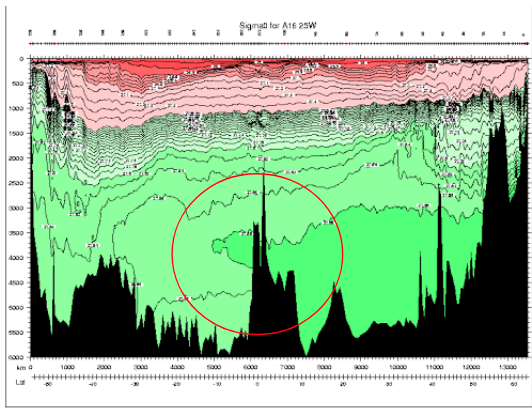
\includegraphics[width=.9\linewidth]{Potential_density/2021-05-01_15-28-04_densinversion.png}
\end{center}

\section{The Neutral Tangent Plane and Helicity}
\label{sec:org2395a0b}
Ok. We've seen how those first two density variables aren't the most neutral but how do we construct a better one. The answer may appear simple; construct a surface that is perfectly neutral upon which water parcels would never experience a restoring force when they travel on it. The thing stopping us is going to be a thorn in our side going forward and it's called helicity. But first, a definition:
\subsection{The Neutral Tangent Plane}
\label{sec:org6bf6efc}
Quickly and informally, we can define the neutral tangent plane as the path between two water columns upon which a water parcel would undergo no restoring force. Practically if we would like to find the neutral tangent plane which passes through (S\textsubscript{0,T}\textsubscript{0,p}\textsubscript{0}) and an adjacent water column with salinity, temperature and pressure (S\textsubscript{i,T}\textsubscript{i,p}\textsubscript{i}), we want to find where \(\rho(S_0,T_0,\frac{p_i+p_0}{2})=\rho(S_i,T_i,\frac{p_i+p_0}{2})\). 

\subsection{Helicity}
\label{sec:orgede0fb0}
In a just world, if we followed the neutral tangent plane throughout the ocean we would be traveling along a perfectly neutral surface which we could label a certain density and go home. But the ocean is a cruel mistress. If you follow the neutral tangent plane through the ocean, hopping from one profile to the next, in a big circle, when you return to where you started you will be at a different pressure forming a big corkscrew or helix and that is helicity. erfectly neutral surfaces are not well-defined meaning that at any given point in space there are multiple (maybe infinite) solutions for their depth. This isn't due to a lack of resolution in our sampling of the ocean, it's just due to the complex multivalued nature of the equation of state. An explanation is out of the scope of this paper but check out( ).  

\section{Neutral surfaces}
\label{sec:org8eb907b}
Helicity. Blech. But we are working oceanographers and helicity will not defeat us! We still want a density variables whose surfaces of constant density are well defined as neutral as possible so we just have to make some tradeoffs! Enter neutral density! Neutral density was made in \_\_ by Jacket and Macdougall and here's how it works. 

\begin{itemize}
\item take reference climatology
\item label it with density, doesn't really matter
\item spread out solving neutral tangent plane. labelling
\item when you see point in between four points solve between each 2.
\end{itemize}

\section{Philosophy}
\label{sec:orge901af2}
Helicity and neutralness what does it mean if helicity is a thing
\begin{itemize}
\item neutral surfaces don't exist and water doesn't travel neatly on surfaces sorry
\item things are mixed
\item we need a density variable cause we like density and if we dont have one our lives are bad
\item the ocean is a cruel cruel mistress
\end{itemize}

I will now give my one sentence impressions of other density variables mostly for fun.

\section{Omega surfaces}
\label{sec:org78bb93d}
Treat surfaces as an optimization problem and minimize error everywhere.

\section{Topobaric Density}
\label{sec:orgbbca689}
Pretend helicity does not exist and do fancy topology to find better density variable. 

\section{In-situ density anomaly surfaces}
\label{sec:org2f8a50e}
Consider difference from a reference salinity and temperature. Very cool and fun two thumbs up.  
\end{document}
